%====================================================================================
\section{Normalidad asintótica e inferencia de muestras grandes}
%====================================================================================

%------------------------------------------------------------------------------------
\subsection{Ley de los grandes numeros}
%------------------------------------------------------------------------------------
\begin{frame}	
	\begin{columns}[onlytextwidth]
			\begin{column}{.45\textwidth}
				\begin{figure}
					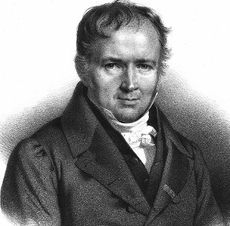
\includegraphics[scale=0.8]{fig/simeon_poisson.jpg}
				\end{figure}
				Siméon Poisson (1781-1840)
			\end{column}
		\hfill
			\begin{column}{.45\textwidth}
				\textit{`No se puede predecir el comportamiento individual, pero si el comportamiento promedio'.}  \\ 
				\bigskip
				La probabilidad que la media muestral se acerque a la media poblacional aumenta con el tamaño de la muestra.
				$$ \bar y_n \xrightarrow{p} \mu $$
			\end{column}
	\end{columns}
\end{frame}

%------------------------------------------------------------------------------------
\subsection{Teorema central del límite}
%------------------------------------------------------------------------------------
\begin{frame}{Teorema central del límite}
	Si $X_1$, $X_2$, ... es una secuencia de V.A. independientes con $E(X_i)=\mu$ y $Var(X_i)=\sigma^2 < \infty$, entonces:
		\begin{gather*}
			\frac{(\bar X_n - \mu)}{\sigma/\sqrt{n}} \xrightarrow{d} N(0,1)\\
			\sqrt{n}\frac{(\bar X_n - \mu)}{\sigma} \xrightarrow{d} N(0,1)\\
			\sqrt{n}(\bar X_n - \mu) \xrightarrow{d} N(0,\sigma^2)
		\end{gather*}
\end{frame}

%------------------------------------------------------------------------------------
\subsection{Teorema de Slutsky}
%------------------------------------------------------------------------------------
\begin{frame}{Teorema de Slutsky}
	Sea $a_n$ y $b_n$ dos variables aleatorias donde la primera cuenta con una distribución asintótica y 
		$$ b_n \xrightarrow{p} b $$
	entonces:
		\begin{enumerate}
			\item $ a_n+b_n \xrightarrow{d} a_n+b $
			\item $ a_n b_n \xrightarrow{d} a_n b $	
		\end{enumerate}
\end{frame}